\documentclass[a4paper, 12pt]{article}
\usepackage[top=2cm, bottom=2cm, left=2.5cm, right=2.5cm]{geometry}

\usepackage[utf8]{inputenc}
\usepackage[brazilian]{babel}
\usepackage{indentfirst}

\usepackage{graphicx}
\usepackage[pdftex]{hyperref}
\graphicspath{ {imagens/} }
\usepackage{xcolor}

%Caracteres Japoneses
\usepackage{CJK}

% Definindo novas cores
\definecolor{verde}{rgb}{0.25,0.5,0.35}
\definecolor{jpurple}{rgb}{0.5,0,0.35}



\begin{document}
	\begin{titlepage} %iniciando a "capa"
		\begin{center} %centralizar o texto abaixo
			{\large Unicamp}\\[0.2cm] %0,2cm é a distância entre o texto dessa linha e o texto da próxima
			{\large Mecatron}\\[0.2cm] % o comando \\ "manda" o texto ir para próxima linha
			{\large Projetos e Consultoria}\\[3.2cm]
			{\bf \huge A cultura do Post Mortem}\\[5.1cm] % o comando \bf deixa o texto entre chaves em negrito. O comando \huge deixa o texto enorme
		\end{center} %término do comando centralizar
		{\large Erik Yuji Goto}\\[10.5cm] % o comando \large deixa o texto grande

		\begin{center}
			{\large Campinas}\\[0.2cm]
			{\large 2021}
		\end{center}
	\end{titlepage} %término da "capa"
	
	\tableofcontents
	
	\newpage
	\section{Cultura Postmortem: Aprendendo a partir de falhas}
	\textit{"O preço do fracasso é a educação". Devin Carraway}\\
	
	Em qualquer tipo de organização as falhas são inevitáveis. E até há a ideia de que aprendemos com nossos fracassos, portanto devemos estar prontos para eles, além de que "errar é humano". Querendo ou não elas estão corretas mesmo que
	 parcialmente, afinal se nunca fracassarmos em algo na vida não conseguiríamos fazer mudanças para incrementar nossa performance.
	
	Apesar de ser importante experienciar fracassos, na realidade da EJ temos uma alta rotatividade(aprox. 2 anos/membro), o que significa que grande parte do conhecimento adquirido por cada pessoa vai embora junto com ela. Portanto, a tendência é a repetição de erros passados, que poderiam ser evitados.
	
	Com o intuito de evitar a repetição constante de erros passados, o Google implementou a cultura do \textbf{postmortem}.
	
	\begin{flushright}
		\textit{"A postmortem is a written record of an incident, its impact, the actions taken to mitigate or resolve it, the root cause(s), and the follow-up actions to prevent the incident from recurring."
	}
	\end{flushright}

	\textbf{O postmortem consiste em documentar as falhas que já ocorreram, incluindo suas causas, e quais ações serão realizadas para evitar que ocorram novamente.} É importante destacar que, redigir um postmortem não é visto como uma punição, mas um aprendizado, e uma contribuição para toda a empresa. 
	
	\subsection{Qual a importância?}
	A \textbf{figura 1} ilustra como deveria ser o processo de aprendizagem a partir de fracassos. Iniciamos com uma meta, em algum momento encontramos dificuldades, aprendemos novos princípios(maneiras de lidar com as falhas), evoluímos(aplicamos os planos de ação), e criamos metas cada vez mais audaciosas. A partir das novas metas encontramos novos obstáculos, ou até mesmo obstáculos que já foram superados, e novamente o ciclo se repete.
	
	A ideia por trás disso é estar constantemente evoluindo, e aumentando o repertório de soluções para cada problema que eventualmente surgir. Quando problemas velhos reaparecerem não precisamos investir tempo e recursos humanos para resolvê-lo.
	\begin{figure}[h]
		\centering
		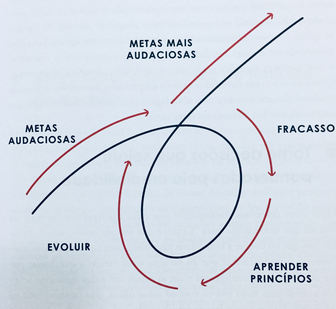
\includegraphics[width=0.3\linewidth]{imagens/princi}
		\caption{Princípios - Ray Dalio}
		\label{fig:princi}
	\end{figure}
	
	A \textbf{figura 2} é o que precisamos evitar, uma evolução praticamente estagnada pois erros velhos são repetidos.
	\begin{figure}[h]
		\centering
		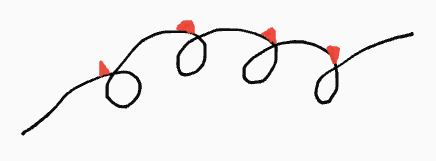
\includegraphics[width=0.5\linewidth]{imagens/princi1}
		\caption{O não aprendizado}
		\label{fig:princi1}
	\end{figure}
	
	\section{Implementação}
	A escrita do documento \textbf{não deve levar muito tempo, nem exigir esforço}, para que não seja uma atividade chata.
	
	\subsection{Gatilhos}
	Criar \textbf{gatilhos claros} sobre o melhor momento para documentar pode ajudar tornar o processo natural. 
	\subsubsection{Execução de Projetos}
	No para a área de excução de projetos, alguns gatilhos sugeridos:
		\begin{itemize}	
			\item Cancelamento de um projeto;
			\item Necessidade de retrabalho de qualquer tipo;
			\item Atraso em mais de um ano para a entrega do projeto;
			\item ...
		\end{itemize}
	
	Além dos gatilhos padrões, \textbf{qualquer pessoa pode requisitar} um postmortem se achar necessário.
	
	\subsection{Compartilhar com a empresa}
	Sempre que um novo documento for redigido é importante que todos tenham conhecimento sobre, ao menos das palavras-chave. Dessa forma, caso outra pessoa passe pelo mesmo problema ela pode se lembrar que aquilo já aconteceu e ler o documento.
	
	\subsection{Revisão do documento}
	Depois de redigido, o documento pode ser mandado para uma pessoa externa revisar. Tendo em mente avaliar os seguintes aspectos:
		\begin{itemize}	
			\item Informações suficiente sobre o incidente chave foi coletado para a posterioridade?
			\item A avaliação sobre os impactos foi completa?
			\item A causa raiz foi identificada?
			\item Os planos de ação são apropriados e os problemas solucionados na prioridade correta?
			\item Compartilhamos as ideias relevantes com os stakeholders corretos?
		\end{itemize}
	
	\section{Boas Práticas}
	Naturalmente, explicitar falhas não é nada fácil. Portanto, a documentação \textbf{NÃO} serve para culpar outras pessoas. Deve-se ter em mente que todos os stakeholders tinham boas pretensões com relação ao projeto. Caso isso não seja passado corretamente para os membros pode-se criar uma \textbf{cultura de ocultação de falhas}, pelo medo da repressão.
	
	Os documentos produzidos devem ser revisitados para que não sejam feitos em vão, se bem feitos com certeza ajudarão em momentos futuros.

	
\end{document}